\documentclass[11pt]{article}

\usepackage[margin=1in]{geometry}

\usepackage{graphicx}

\usepackage{booktabs}

\usepackage{amsmath}

\usepackage{hyperref}

\usepackage{float}

\newif\ifdraft
\drafttrue

\title{From Global Event to Discursive Field: A Computational Analysis of International Yoga Day, 2014--2026}


\usepackage{authblk}

\author[1]{Patrick S. D. McCartney\thanks{ORCID: 0000-0002-3222-9366}}

\affil[1]{Nanzan University Anthropological Institute}
\affil[2]{Australian National University}
\affil[3]{Manipal Academy of Higher Education}

\date{\today}



\begin{document}



\maketitle



\begin{abstract}



Existing scholarship on the International Day of Yoga (IDY) has largely focused on public diplomacy, cultural branding,
and health promotion. However, relatively little attention has been given to the evolution of discourse surrounding the
event itself. This study presents a longitudinal computational analysis of 509 transcripts spanning 2014--2026. Using a
Discourse Structure Index (DSI), cluster analysis, ANOVA, interaction models, and mixed-effects regression, the study
identifies four distinct discourse communities and demonstrates significant temporal change in discourse structure.
Results indicate increasing differentiation among institutional actors and uneven developmental trajectories across
discourse clusters. The findings suggest that the IDY has evolved into a heterogeneous discursive field shaped by
processes of mediatization and institutionalization.


\end{abstract}



\section{Introduction}



The International Day of Yoga (IDY) was established by the United Nations General Assembly in 2014 and first observed in
2015. While it has become a globally recurring cultural and media event, which appears to have superfically remained
constant in the form of a public event centred around promoting yoga culture - and by proxy the Indian state – much of
the academic literature has focused on the events relation to diplomacy, public health, and cultural nationalism. In
contrast, less attention has been paid to how IDY is communicated across media environments. Therefore, this paper
investigates the structural evolution of IDY discourse using computational methods. It begins by asking the following
questions:


\begin{enumerate}

\item Do discourse clusters differ significantly in discourse structure?

\item Does discourse structure change over time?

\item Do clusters exhibit different temporal trajectories?

\end{enumerate}




\section{Literature Review}


Recent policy-oriented assessments have highlighted the rapid institutional expansion of yoga following the establishment of
IDY, documenting growth across public health, education, workplace wellness, digital technologies, and research
infrastructure. These assessments argue that yoga has increasingly become embedded within diverse institutional domains while also
calling for more longitudinal and context-sensitive forms of research. The present study responds to this need by examining
International Day of Yoga discourse as an evolving system of institutional communication spanning 2014--2026.
Therefore, while recent assessments of the IDY emphasize the need for longitudinal, data-driven,
and sociologically informed research [[Prasad, Ankeetaa Mahesshwari and Kaur 2025]], computational analyses of the 
evolution of IDY discourse remain scarce. This study addresses that gap through the analysis of 509 transcripts spanning 2014–2026.




\subsection{Yoga, Modernity, and Global Circulation}


Modern yoga is widely understood as a hybrid cultural formation shaped by colonial encounters, transnational
circulation, physical culture movements, and global wellness industries. Rather than a singular tradition, yoga operates
as a contested field of meaning shaped by competing institutional, spiritual, and political claims. For example, the
theme for IDY 2019 was climate action. Embedded within this phrase is the claim that a under-defined yogic lifestyle can
help prevent climate change. The perceived transformative potential relates to an apparent power to heal humanity’s
relationship with the earth. It is assumed that through adopting a generic yogic lifestyle that the individual consumer
would naturally develop more sustainable attitudes and practices.

For example, adopting yoga is considered essential to creating \textit{Low Carbon Lifestyles: Right Choices for our Planet} [[MOEFCC 2016]].
Scaling this up to the level of every global citizen adopting such a lifestyle is then considered by Prime Minister Narendra Modi to encompass a powerful instrument to
tackle climate change through “changing our lifestyle and creating consciousness,” and also a path to wellness that will
somehow make us better individuals in “thought, action, knowledge and devotion" [[see Indian Diplomacy 2017; United Nations 2016a; United Nations 2016b; United Nations 2019]].
This is where lifestyle and policy merge. For example, the Indian government's Ministry of Environment, Forest and Climate Change's 
website has quotes from a speech that Modi gave to promote the Mission Life project to the world at the \textit{26th UN Climate Change 
Conference of the Parties (COP26)} in Glasgow. Modi stated that "Mission Life can become a mass movement of Environmental Conscious Lifestyle.
 [...] Mission Lifestyle for Environment recognises that Indian culture and living traditions are inherently sustainable.
The importance of conserving our precious natural resources and living in harmony with nature are emphasised in our ancient scriptures.
The need of the hour is to tap into that ancient wisdom and spread the message to as many people as possible. Mission Life 
seeks to channel the efforts of individuals and communities into a global mass movement of positive behavioural change" [[MOEFCC 2026]].



\subsection{International Yoga Day and Cultural Diplomacy}


Since its inception in 2015, the International Day of Yoga (IDY) has frequently been interpreted as an instrument of
cultural diplomacy and soft power. For example, in the executive summary of the \textit{The Research Impact of 
International Day of Yoga: A Scientometric Analysis of Yoga's Global Influence} [[Prasad, Ankeetaa Mahesshwari and Kaur 2025]], "IDY has become far more 
than a ceremony, it has successfully managed to amplify wellness narratives, encourage mass participation, 
and provide visibility to yoga’s enduring and universal relevance" [[Prasad, Ankeetaa Mahesshwari and Kaur 2025]].

Scholars have argued that the IDY campaign acts as a mechanism through which India projects cultural heritage, promotes wellness narratives, and
enhances its visibility within global public discourse [[Kaur, Ganguli and Singh 2025]]. At the same time, critical
scholars have examined the relationship between IDY, nationalism, identity politics, and state-sponsored cultural
narratives [[McCartney 2018; McCartney 2019a; McCartney 2019b; McCartney 2025; McCartney 2026]]. Other studies have examined how yoga has been mobilized as a 
resource of state branding and international influence, highlighting the relationship between yoga, Hindutva, and 
India's global image [[Gautam and Droogan 2018; Miller 2020; Samal 2020]].

Despite the global prominence of IDY, the dedicated scholarly literature remains relatively limited and highly
concentrated. A hand-coded bibliographic survey conducted for the present study identified only 26 publications directly
focused on IDY. The majority of these publications are concerned with health promotion, therapeutic applications, and
wellness outcomes (n = 12), while a further eight publications primarily document commemorative events, conferences, and
public participation initiatives. By contrast, analytical scholarship addressing political discourse, cultural
diplomacy, nationalism, media representation, and broader social implications constitutes a comparatively small
proportion of the field (n = 6).

This distribution suggests that existing scholarship has largely approached IDY as a public health initiative or
commemorative event rather than as a complex communicative phenomenon. Studies such as \textit{The Transformative Impact
of the International Day of Yoga} [[Manjunath 2023]], \textit{Impact Assessment of International Day of Yoga}
[[Mohan,Vadiraja, Moirangthem, et al. 2024]], and the Kolar conference proceedings emphasize health promotion,
participation, and wellness outcomes [[Bhattacharyya, Patil and Muninarayana 2015; Patil, Venkatarathnamma and RamchandraRao 2016]]. 

In contrast, a smaller body of work has situated IDY within broader debates
concerning soft power, diplomacy, nationalism, and political symbolism. Notable examples include \textit{The
International Yoga Day, Political Discourse, and Soft Power Game in India} [[Samal 2020]], \textit{Choreographing
Tolerance: Narendra Modi, Hindu Nationalism, and International Yoga Day} [[Kedhar 2020]], and \textit{The
Unintended Consequences of International Day of Yoga} [[McCartney 2018]].

An important distinction emerges when citation counts are considered. Although health-oriented and promotional studies
constitute the numerical majority of publications, several of the most influential contributions focus on political
discourse, nationalism, and cultural diplomacy. The most highly cited publication in the field, \textit{Choreographing
Tolerance} [[Kedhar 2020]], examines the relationship between IDY and Hindu nationalism, while other highly
cited studies investigate the diplomatic and political dimensions of the initiative [[Samal 2020; McCartney 2018]]. 
Consequently, the dominant publication profile of the field differs from the topics that have attracted
the greatest scholarly attention.


Taken together, the literature reveals two broad tendencies. The first consists of promotional and descriptive accounts
that document participation, health outcomes, and public engagement. The second comprises analytical and critical
scholarship that situates IDY within wider discussions of soft power, nationalism, statecraft, and global cultural
politics. While these studies have generated important insights into the ideological, diplomatic, and symbolic
dimensions of IDY, relatively little attention has been devoted to the systematic analysis of discourse itself. In
particular, longitudinal computational investigations of how IDY communication evolves across institutional actors,
media environments, and time remain rare.


The present study addresses this gap through a corpus-based analysis of 509 transcripts spanning the period 2014--2026.
Rather than evaluating yoga as a therapeutic intervention or assessing the effectiveness of diplomatic initiatives, it
examines the emergence, differentiation, and temporal evolution of discourse communities within the broader
communicative field surrounding International Yoga Day.




\subsection{The Prevalence of Normative Scholarship}



A substantial portion of the IDY literature is normative or promotional, emphasizing health benefits, participation, or
cultural value. While informative, this literature often assumes the value of IDY rather than empirically analyzing its
discourse. This study instead treats IDY discourse as an object of analysis.



\subsection{Mediatization and Institutionalization}



Mediatization theory suggests that recurring cultural events become shaped by media logics, leading to increased
standardization and differentiation of communication [[Hjarvard 2008]]. Institutionalization theory further predicts that repeated events
stabilize into structured communicative regimes [[Stavolo 2026]]. Applied to IDY, this implies increasing differentiation among discourse communities over time.



\subsection{Computational Discourse Analysis}



Computational approaches enable large-scale analysis of discourse structures 
across time. However, few studies have applied such methods to IDY. 
This study addresses this gap.

Computational approaches to discourse have increasingly
emphasized the analysis of large textual corpora as evolving social
systems rather than collections of isolated texts. Research in
computational discourse analysis and computational sociology has
demonstrated the value of clustering, text mining, and longitudinal
modelling for identifying discourse communities, tracking cultural
change, and examining institutional communication at scale.

The present study brings these literatures together by treating
International Yoga Day discourse as a longitudinal corpus of
institutional communication. Rather than analysing individual texts or
elite narratives, it examines how discourse communities emerge,
differentiate, and evolve over time through computational analysis of
509 transcripts spanning 2014--2026.

This study treats IDY discourse as an evolving social system whose structural 
properties can be observed computationally (Keuschnigg, Lovsjö and Hedström 2018). 
This contribution substantiates the first large-scale longitudinal analysis of IDY 
discourse [[Camilleri and Miah 2021]]. Methodologically, it contrib>. In service of
 the above mentioned questions, this paper attends to text analysis, clustering, 
longitudinal modeling, and institutional differentiation [[Bonikowski and Nelson 2022]].
 So too, the use of DSI and cluster trajectories toward comptational text analysis can be
 used to develop and test sociological theory rather than merely classify text
 [[Hurtado Bodel, Keuschnigg, Macanovic, et al. 2026]]. Theoretically, it contributes evidence that 
global commemorative discourse evolves through institutional differentiation rather than conve>

 

\section{Corpus and Methodology}



\subsection{Corpus Identification and Construction}



The corpus analysed in this study was constructed through an iterative process of digital data collection, automated
scraping, transcript extraction, and corpus validation. Unlike studies based on pre-existing institutional archives, the
present dataset was assembled specifically for the purpose of investigating the evolution of discourse surrounding
International Yoga Day (IDY) between 2014 and 2026.


Corpus construction began with extensive exploratory searches across YouTube, which has served as one of the principal
platforms through which governments, public institutions, yoga organisations, news agencies, educational institutions,
and private individuals have documented and disseminated IDY-related activities. Initial searches employed a range of
keywords and phrases, including `International Day of Yoga,'' `International Yoga Day,'' `IDY,'' `Yoga Day,'' and
related multilingual variants. These searches returned thousands of videos varying considerably in relevance, quality,
format, language, and institutional affiliation.


A major challenge involved distinguishing videos directly related to International Yoga Day from the much larger body of
general yoga content available on the platform. Multiple iterations of collection and filtering procedures were
therefore developed. Early retrieval stages produced substantial quantities of irrelevant material, including general
yoga instruction videos, wellness content, commercial yoga promotion, and unrelated discussions of yoga philosophy. To
improve precision, search strategies were repeatedly refined through keyword expansion, metadata filtering, transcript
inspection, and manual validation.


Several generations of custom Python scripts were developed during the course of the project. These scripts automated
video discovery, metadata collection, subtitle retrieval, transcript extraction, duplicate detection, and corpus
management. Collection procedures were repeatedly revised in response to changes in YouTube's interface, inconsistencies
in subtitle availability, variable metadata quality, and occasional retrieval failures. Transcript recovery combined
available subtitle files with automated extraction procedures where necessary, producing a substantially larger corpus
than would have been obtainable through manual collection alone.


The resulting dataset underwent extensive cleaning and validation. Duplicate videos were removed, transcript quality was
assessed, corrupted or incomplete files were excluded, and metadata fields were standardized. Additional validation
procedures were implemented to ensure that retained videos were genuinely related to International Yoga Day rather than
to yoga more generally. Manual inspection of sampled transcripts and metadata records was conducted throughout the
collection process to verify corpus quality and relevance.


The final corpus consists of 509 transcripts spanning the period 2014--2026. The dataset includes governmental
broadcasts, news coverage, institutional events, educational programmes, yoga demonstrations, public-awareness
campaigns, speeches, interviews, and commemorative activities associated with International Yoga Day. Taken together,
these materials provide a longitudinal record of how IDY has been represented, promoted, interpreted, and discussed
across diverse media environments over more than a decade.


\subsection{Analytical Workflow}



Following corpus construction, transcripts were cleaned and transformed into document-level representations suitable for
computational analysis. Texts were embedded using sentence-level semantic representations and grouped using unsupervised
clustering techniques. This procedure enabled the identification of recurrent discourse communities within the corpus
without imposing predetermined thematic categories.


To investigate structural differences between discourse communities, a Discourse Structure Index (DSI) was developed.
The DSI provides a quantitative measure of discursive positioning across documents and clusters, allowing comparison
between different forms of IDY communication. Cluster-level patterns, temporal trends, and interaction effects were
examined through descriptive statistics, analysis of variance, ordinary least-squares regression, and mixed-effects
modelling.


The primary objective of the analytical workflow was not simply to identify topics, but to examine how distinct
discourse communities emerged, evolved, and interacted across time. By combining computational clustering with
longitudinal statistical analysis, the study provides a framework for understanding the institutionalization and
diversification of International Yoga Day discourse between 2014 and 2026.






\subsection{Corpus}



The dataset contains 509 transcripts collected between 2014 and 2026 across media, governmental, educational, wellness, and other institutional channels.



\begin{table}[H]

\centering

\begin{tabular}{lr}

\toprule

Category & Count \\

\midrule

News & 108 \\

State & 76 \\

Wellness & 17 \\

Education & 6 \\

Religious & 3 \\

Other & 299 \\

\bottomrule

\end{tabular}

\caption{Corpus composition by channel type}

\end{table}



\subsection{Methods}

The analytical strategy is structured explicitly around the three hypotheses, ensuring that each inferential claim is supported by a corresponding statistical procedure.

\begin{itemize}

\item \textbf{H1: Structural differentiation of discourse clusters.}  
To test whether discourse clusters differ significantly in Discourse Structure Index (DSI), we employ one-way analysis of variance (ANOVA), with cluster membership as the independent factor and DSI as the dependent variable. Where significant omnibus effects are observed, post-hoc pairwise comparisons are conducted using Tukey’s Honest Significant Difference (HSD) test to identify specific inter-cluster differences.

\item \textbf{H2: Temporal change in discourse structure.}  
To assess whether DSI changes over time, we estimate ordinary least squares (OLS) regression models with year (or time index) as the primary predictor of DSI. This allows us to evaluate linear temporal trends in discourse structure across the full corpus. Robust standard errors are used where appropriate to account for heteroskedasticity in time-series observations.

\item \textbf{H3: Heterogeneous temporal trajectories across clusters.}  
To examine whether discourse clusters exhibit distinct developmental trajectories, we estimate interaction models that include both time and cluster membership. Specifically, we fit OLS regression models with interaction terms between cluster indicators and time, allowing slopes to vary across clusters. In addition, mixed-effects models are employed to account for repeated observations within clusters and to model unobserved cluster-level heterogeneity.

\end{itemize}


\section{Hypotheses}

This study advances three primary hypotheses concerning the structure and evolution of discourse within International Yoga Day (IDY) communication. These hypotheses are grounded in the assumption that institutional context and temporal dynamics jointly shape discursive form and intensity.

\begin{itemize}

\item \textbf{H1 (Structural differentiation):} Discourse clusters exhibit statistically significant differences in Discourse Structure Index (DSI), reflecting systematic variation in rhetorical organisation across institutional contexts (e.g., state, media, wellness, education).

\item \textbf{H2 (Temporal evolution):} DSI values change significantly over time, indicating that discourse becomes more or less structurally complex as International Yoga Day communication stabilises and institutionalises across the 2014--2026 period.

\item \textbf{H3 (Cluster-specific trajectories):} Temporal trajectories of DSI differ across discourse clusters, such that institutional domains evolve along distinct developmental pathways rather than converging toward a single unified discourse structure.

\end{itemize}

Together, these hypotheses conceptualise discourse as a dynamic and institutionally embedded system rather than a static set of thematic categories.


\section{Results}

\subsection{H1: Structural differentiation across discourse clusters}

Consistent with H1, we find strong evidence that discourse clusters differ significantly in Discourse Structure Index (DSI). A one-way ANOVA indicates a robust overall effect of cluster membership on DSI. Post-hoc Tukey HSD comparisons further reveal that most cluster pairs differ significantly from one another, indicating systematic structural differentiation across institutional discourse types.

These results suggest that discourse clusters are not merely topical groupings but represent structurally distinct forms of communication, shaped by institutional context and communicative purpose.

\subsection{H2: Temporal change in discourse structure}

In support of H2, regression analyses show that DSI exhibits a statistically significant relationship with time. The OLS model indicates a clear temporal trend in discourse structure over the 2014–2026 period, suggesting that communicative form evolves as International Yoga Day discourse becomes more institutionalised and globally diffused.

This pattern indicates that discourse structure is not static, but responsive to broader temporal processes such as institutional consolidation and media diffusion.

\subsection{H3: Cluster-specific temporal trajectories}

Supporting H3, interaction models reveal that temporal changes in DSI differ significantly across discourse clusters. The inclusion of cluster-by-time interaction terms improves model fit and demonstrates heterogeneous slopes across institutional categories.

Mixed-effects models further confirm that clusters exhibit distinct developmental trajectories over time, with some clusters showing increasing structural complexity while others remain stable or decline. This indicates that discourse evolution is not uniform, but segmented along institutional lines.


\subsection{Cluster Differences}



Cluster differences are highly significant:



\begin{equation*}
F = 142.62,\quad p < 0.001
\end{equation*}


Tukey tests confirm strong pairwise differences between most clusters.



\subsection{Institutional Structure of Clusters}



A chi-square test indicates strong alignment between clusters and channel types:


\begin{equation*}
X = 91.98, \quad p < 0.001
\end{equation*}

This suggests that clusters reflect institutional differentiation.



\subsection{Temporal Trends}



Overall discourse structure increases over time:



\begin{equation*}
\rho = 0.248,\quad p < 0.001
\end{equation*}



\subsection{Cluster-Specific Trends}



Cluster trajectories differ significantly:



\begin{itemize}

\item Cluster 4: strong positive trend

\item Cluster 0: moderate positive trend

\item Cluster 6: strong positive trend

\item Cluster 2: weak/non-significant trend

\end{itemize}



\subsection{Interaction Model}

Regression results confirm differential slopes across clusters, indicating heterogeneous temporal development. 
In other words, the way discourse structure changes over time is not the same for all clusters.
This is tested using interaction terms between cluster membership and time in the regression model. 
These interaction effects allow the slope of the Discourse Structure Index (DSI) to vary by cluster 
rather than assuming a single shared trend across the entire corpus.The results show that these interaction 
terms are statistically significant, confirming that clusters follow distinct temporal trajectories. 
Practically, this means that some discourse communities become more structurally complex over time, while 
others remain stable or change at different rates. Instead of a single unified developmental pattern, the 
system is better characterised as a set of parallel but divergent evolutionary paths across institutional discourse types.


\subsection{Mixed-Effects Model}



\begin{table}[H]

\centering

\begin{tabular}{lrr}

\toprule

Model & AIC & BIC \\

\midrule

OLS Full & 672.48 & 706.34 \\

Mixed Effects & 653.45 & 695.78 \\

\bottomrule

\end{tabular}

\caption{Model comparison}

\end{table}



Mixed-effects models outperform OLS, indicating strong channel-level variance.



\section{Discussion}

\subsection{H1: Structural differentiation and institutional embedding}

The findings supporting H1 demonstrate that discourse clusters are not merely topical 
aggregations but structurally differentiated communicative regimes. Significant variation 
in Discourse Structure Index (DSI) across clusters suggests that institutional context 
plays a central role in shaping rhetorical organisation. This supports the interpretation of 
International Yoga Day discourse as a multi-centred communicative system, in which state, media, 
educational, and wellness actors produce systematically distinct forms of structured communication 
rather than converging on a unified discourse style.

\subsection{H2: Temporal evolution and institutionalisation}

The results supporting H2 indicate that discourse structure evolves significantly over time. 
The observed temporal trends in DSI suggest a gradual reconfiguration of communicative 
practices across the 2014–2026 period.

This pattern is consistent with processes of institutionalisation, in which repeated annual 
articulation of International Yoga Day leads to increasing stabilisation, routinisation, 
and formalisation of discourse practices. However, the presence of directional change rather 
than convergence suggests that institutionalisation does not produce uniformity, but structured evolution.

\subsection{H3: Divergent trajectories and discursive fragmentation}

The findings supporting H3 show that discourse clusters follow heterogeneous temporal trajectories. 
Rather than converging toward a single stable discourse structure, clusters exhibit distinct developmental 
pathways over time.

This divergence suggests that institutional domains maintain internal logics of communication that persist 
even under conditions of shared global framing. The resulting pattern is one of structured fragmentation: 
a system in which discourse evolves, but does so along multiple, institutionally anchored trajectories.

\subsection{Synthesis}

Taken together, the results indicate that International Yoga Day discourse operates as a dynamically 
structured system shaped by both institutional differentiation and temporal evolution. Rather than a 
unified global discourse, the corpus reveals a layered configuration of semi-autonomous discourse 
regimes that evolve along distinct trajectories while remaining loosely coupled within a shared symbolic event.


\subsection{Discursive Institutionalization}


The findings suggest that IDY has undergone a process of discursive institutionalization during the period under
investigation. Across the corpus, discourse becomes increasingly differentiated, organized, and structured over time.
This pattern is reflected in both the clustering results and the temporal analyses, which indicate that distinct
communicative forms emerge and stabilize as IDY develops from a newly established international observance into a
recurring global event.


Institutionalization refers not merely to the growth of participation but to the emergence of relatively stable
communicative practices, expectations, and organizational forms. In the early years of the corpus, discourse surrounding
IDY exhibits comparatively low levels of differentiation and frequently emphasizes foundational themes such as
awareness, participation, legitimacy, and public promotion. Over time, however, discourse communities become
increasingly specialized. Different actors begin to emphasize distinct objectives, including public health, education,
diplomacy, cultural heritage, community engagement, and governmental policy. This diversification suggests that IDY has
evolved from a singular commemorative initiative into a broader institutional field containing multiple communicative
centres.


These findings are consistent with theories of institutionalization, which predict increasing differentiation and
specialization as social initiatives mature and become embedded within organizational structures. Rather than remaining
a one-time symbolic event, IDY appears to have generated a durable communicative infrastructure that reproduces itself
annually through media coverage, public events, governmental initiatives, and institutional participation.


\subsection{Emergence of a Discursive Field}



The clustering analysis demonstrates that IDY is best understood not as a unified discourse but as a heterogeneous
discursive field composed of multiple actors operating according to different communicative logics. Although all corpus
documents are connected through reference to International Yoga Day, they nevertheless exhibit substantial variation in
linguistic structure, thematic emphasis, and discursive orientation.


This finding challenges representations of IDY as a singular global movement or coherent ideological project. Instead,
the corpus suggests the coexistence of multiple overlapping discourse communities. Government agencies employ IDY to
communicate policy objectives and national initiatives. Educational institutions emphasize awareness and learning.
Health-oriented actors focus on wellness outcomes and therapeutic benefits. Media organizations frame IDY as a
newsworthy event, while cultural organizations position it within broader narratives of heritage, identity, and social
participation.


From this perspective, International Yoga Day functions as a discursive arena within which diverse actors negotiate
meaning rather than as a single unified message transmitted from a central source. The resulting communicative ecology
is therefore characterized by plurality, contestation, and differentiation. This interpretation aligns with broader
approaches in discourse studies that view public events as sites of meaning-making rather than as vehicles for the
transmission of fixed ideological content.


The identification of distinct discourse communities is particularly important because it demonstrates that IDY has
become capable of accommodating multiple institutional agendas simultaneously. Such flexibility may help explain its
continued expansion and durability across different national and organizational contexts.


\subsection{Uneven Temporal Development}



A second important finding concerns the uneven temporal development of discourse communities. The longitudinal analyses
reveal that institutionalization is not occurring uniformly across the corpus. Some clusters display strong positive
temporal trajectories, while others remain relatively stable or exhibit more limited rates of change.


This result suggests that different sectors of the IDY communicative field are evolving according to distinct
developmental logics. Certain discourse communities appear to be rapidly expanding and becoming more structurally
differentiated, whereas others have reached a comparatively stable configuration. The significant interaction effects
observed in both regression and mixed-effects models indicate that temporal change is conditioned by cluster membership
rather than operating as a uniform process affecting all discourse equally.


The existence of uneven developmental trajectories has important theoretical implications. It suggests that
institutionalization should not be conceptualized as a singular linear process. Rather, IDY appears to consist of
multiple partially autonomous discourse communities, each responding differently to changing political, social,
cultural, and media conditions. This finding is consistent with contemporary theories of institutional fields, which
emphasize heterogeneity, competition, and differentiated rates of organizational change.


Moreover, the results imply that future analyses of IDY should move beyond aggregate measures of growth or participation
and instead examine the specific trajectories of individual discourse communities. Such an approach may provide a more
nuanced understanding of how cultural initiatives evolve through time.


\subsection{Beyond Advocacy Scholarship}



The present study also contributes to the emerging literature on International Yoga Day itself. Existing scholarship has
tended to focus on three primary themes: health promotion, cultural diplomacy, and political interpretation. Much of
this work is either explicitly promotional, documenting the benefits of yoga and public participation, or descriptive,
reporting events and institutional activities associated with IDY. A smaller but influential body of scholarship has
examined questions of nationalism, soft power, and political symbolism.


While these contributions have generated valuable insights, relatively little research has treated IDY as an empirical
object of discourse analysis. The dominant emphasis has been on evaluating the initiative's health outcomes, diplomatic
significance, or ideological implications rather than investigating the communicative structures through which those
meanings are produced and circulated.


The present study adopts a different approach. Rather than asking whether IDY is beneficial, effective, or politically
desirable, it examines how discourse surrounding IDY is organized and how that organization changes over time. By
combining corpus construction, unsupervised clustering, longitudinal analysis, and statistical modelling, the study
shifts attention from normative evaluation to empirical investigation.


This distinction is important because it allows IDY to be analysed as a communicative system in its own right. From this
perspective, questions concerning health promotion, nationalism, cultural diplomacy, or public participation become
observable components of a broader discursive field rather than predetermined explanatory frameworks. Such an approach
opens new possibilities for the study of contemporary cultural initiatives, public rituals, and globally mediated
commemorative events.


More broadly, the findings demonstrate the value of computational approaches for investigating large-scale cultural
phenomena. By analysing discourse longitudinally and at scale, researchers can move beyond isolated case studies and
examine the processes through which institutional narratives emerge, stabilize, and transform over time. In this
respect, International Yoga Day provides a useful case study of how cultural, political, and health-related discourses
become institutionalized within contemporary digital media environments.


\section{Limitations}



Several limitations should be acknowledged when interpreting the findings of this study.



First, the corpus exhibits uneven temporal coverage across the study period. Although the final dataset spans the years
2014--2026, the number of available transcripts varies considerably between years. Early years of the corpus contain
relatively few documents, while later years are represented by substantially larger samples. This imbalance reflects
both the historical development of International Yoga Day itself and the availability of digital media content.
Consequently, yearly comparisons should be interpreted cautiously, particularly for years with limited observations.


Second, the corpus is platform-dependent. The dataset was constructed primarily from YouTube transcripts and therefore
reflects communicative practices that are recorded, archived, and distributed through a specific digital media
environment. While YouTube provides extensive coverage of IDY-related activities, it does not capture the entirety of
the communicative field. Important forms of discourse circulating through television broadcasts, print media,
governmental documents, social media platforms, organizational reports, and offline events remain outside the scope of
the present analysis. The corpus should therefore be understood as a substantial but necessarily partial representation
of IDY discourse.


Third, the dataset exhibits a degree of linguistic bias. Although efforts were made to include multilingual material
where available, the final corpus is disproportionately composed of English-language transcripts due to the greater
availability and accessibility of English subtitles and transcripts on the platform. As a result, the findings may
underrepresent communicative practices occurring in Hindi and other regional languages, as well as forms of discourse
intended primarily for local rather than international audiences.


Fourth, the Discourse Structure Index (DSI) developed in this study is designed to capture structural variation within
discourse rather than semantic meaning in a narrow sense. The index identifies patterns of differentiation,
organization, and positioning among discourse communities, but it does not directly measure ideological content,
sentiment, persuasion, or political orientation. Consequently, DSI values should be interpreted as indicators of
discursive structure rather than as direct measures of substantive meaning.


Fifth, the study relies upon automated transcript extraction and computational text-processing procedures. Although
extensive cleaning, validation, and quality-control measures were implemented throughout corpus construction,
transcript-based research inevitably contains a degree of noise arising from subtitle errors, transcription
inaccuracies, metadata inconsistencies, and platform-specific artefacts. While these factors are unlikely to alter the
overall patterns identified in the analysis, they may influence individual documents and local cluster assignments.


Finally, the clustering procedures employed in this study represent one possible interpretation of the latent structure
of the corpus. Alternative embedding models, clustering algorithms, preprocessing strategies, or parameter selections
may produce somewhat different cluster boundaries. The objective of the analysis is therefore not to identify a single
definitive classification of IDY discourse, but rather to reveal robust patterns of differentiation and temporal
development within a large and heterogeneous corpus.


Despite these limitations, the consistency of the observed temporal trends across multiple statistical procedures,
including analysis of variance, regression modelling, and mixed-effects models, suggests that the principal findings are
unlikely to be artefacts of a particular methodological choice.


\section{Conclusion}



This study has examined the evolution of International Yoga Day discourse through a longitudinal corpus of 509
transcripts spanning the period 2014--2026. Using unsupervised clustering, a Discourse Structure Index, and a series of
statistical analyses, the study investigated how communicative practices associated with IDY have changed over time and
how different discourse communities have developed within the broader communicative field.


The findings indicate that International Yoga Day has evolved from a newly established global observance into a
heterogeneous and increasingly differentiated discursive field. Rather than constituting a singular global narrative,
IDY is characterized by multiple discourse communities associated with governmental institutions, media organizations,
educational initiatives, health-promotion activities, and broader cultural projects. These communities exhibit distinct
communicative structures and follow different developmental trajectories through time.


The longitudinal analyses further suggest that the institutionalization of IDY is an uneven process. While some
discourse communities display strong positive temporal trends and increasing structural differentiation, others remain
comparatively stable. This pattern indicates that institutionalization should not be understood as a uniform process
affecting all actors equally. Instead, the communicative field surrounding IDY appears to consist of multiple partially
autonomous domains that evolve according to different organizational and media logics.


The study also contributes to the emerging scholarship on International Yoga Day by shifting attention away from
predominantly normative debates concerning health benefits, public participation, or diplomatic effectiveness. Rather
than evaluating whether IDY succeeds as a health intervention, cultural initiative, or soft-power strategy, the present
analysis examines how discourse surrounding the event is organized, reproduced, and transformed over time. In doing so,
it demonstrates the value of treating IDY as an empirical object of discourse analysis rather than solely as a
political, diplomatic, or wellness phenomenon.


More broadly, the findings contribute to ongoing discussions concerning mediatization, institutionalization, and the
formation of contemporary cultural events within digital media environments. International Yoga Day provides a useful
case through which to observe how globally visible commemorative initiatives generate durable communicative
infrastructures, attract diverse institutional actors, and produce increasingly differentiated forms of discourse. The
emergence of these discourse communities illustrates how cultural events become stabilized, reproduced, and transformed
through recurring cycles of media production and institutional participation.


The robustness of these findings is further supported by the statistical modelling results. In addition to descriptive
analyses and ordinary least-squares regression, a mixed-effects model was estimated to account for variation associated
with individual sources within the corpus. Model comparison indicated that the mixed-effects specification provided a
superior fit to the data, suggesting that the observed temporal patterns cannot be attributed solely to a small number
of prolific channels or content producers. Rather, the results persist even after accounting for hierarchical variation
within the dataset, strengthening confidence that the identified trends reflect broader processes of discursive
development and institutionalization across the IDY communicative field.


Future research may extend this work by incorporating additional platforms, expanding multilingual coverage, conducting
comparative analyses with other United Nations observances, or integrating qualitative discourse analysis with
computational approaches. Such research would further illuminate the processes through which global cultural initiatives
are communicated, contested, and institutionalized in an increasingly networked media landscape.


Taken together, the results suggest that International Yoga Day is best understood not as a singular event, policy
initiative, or unified global message, but as an evolving communicative ecosystem characterized by multiple discourse
communities, institutional actors, and developmental trajectories. Over the first decade of its existence, this
ecosystem has become increasingly differentiated and structurally complex, reflecting broader processes of mediatization
and institutionalization within contemporary digital culture. The study therefore contributes both a methodological
framework for the computational analysis of large-scale cultural discourse and an empirical account of how a globally
visible cultural initiative becomes stabilized, reproduced, and transformed through communication over time.




\clearpage



\section*{Figures}



\begin{figure}[H]

\centering

\includegraphics[width=\textwidth]{figures/dsi-cluster-distribution.png}

\caption{DSI distribution across clusters}

\end{figure}



\begin{figure}[H]

\centering

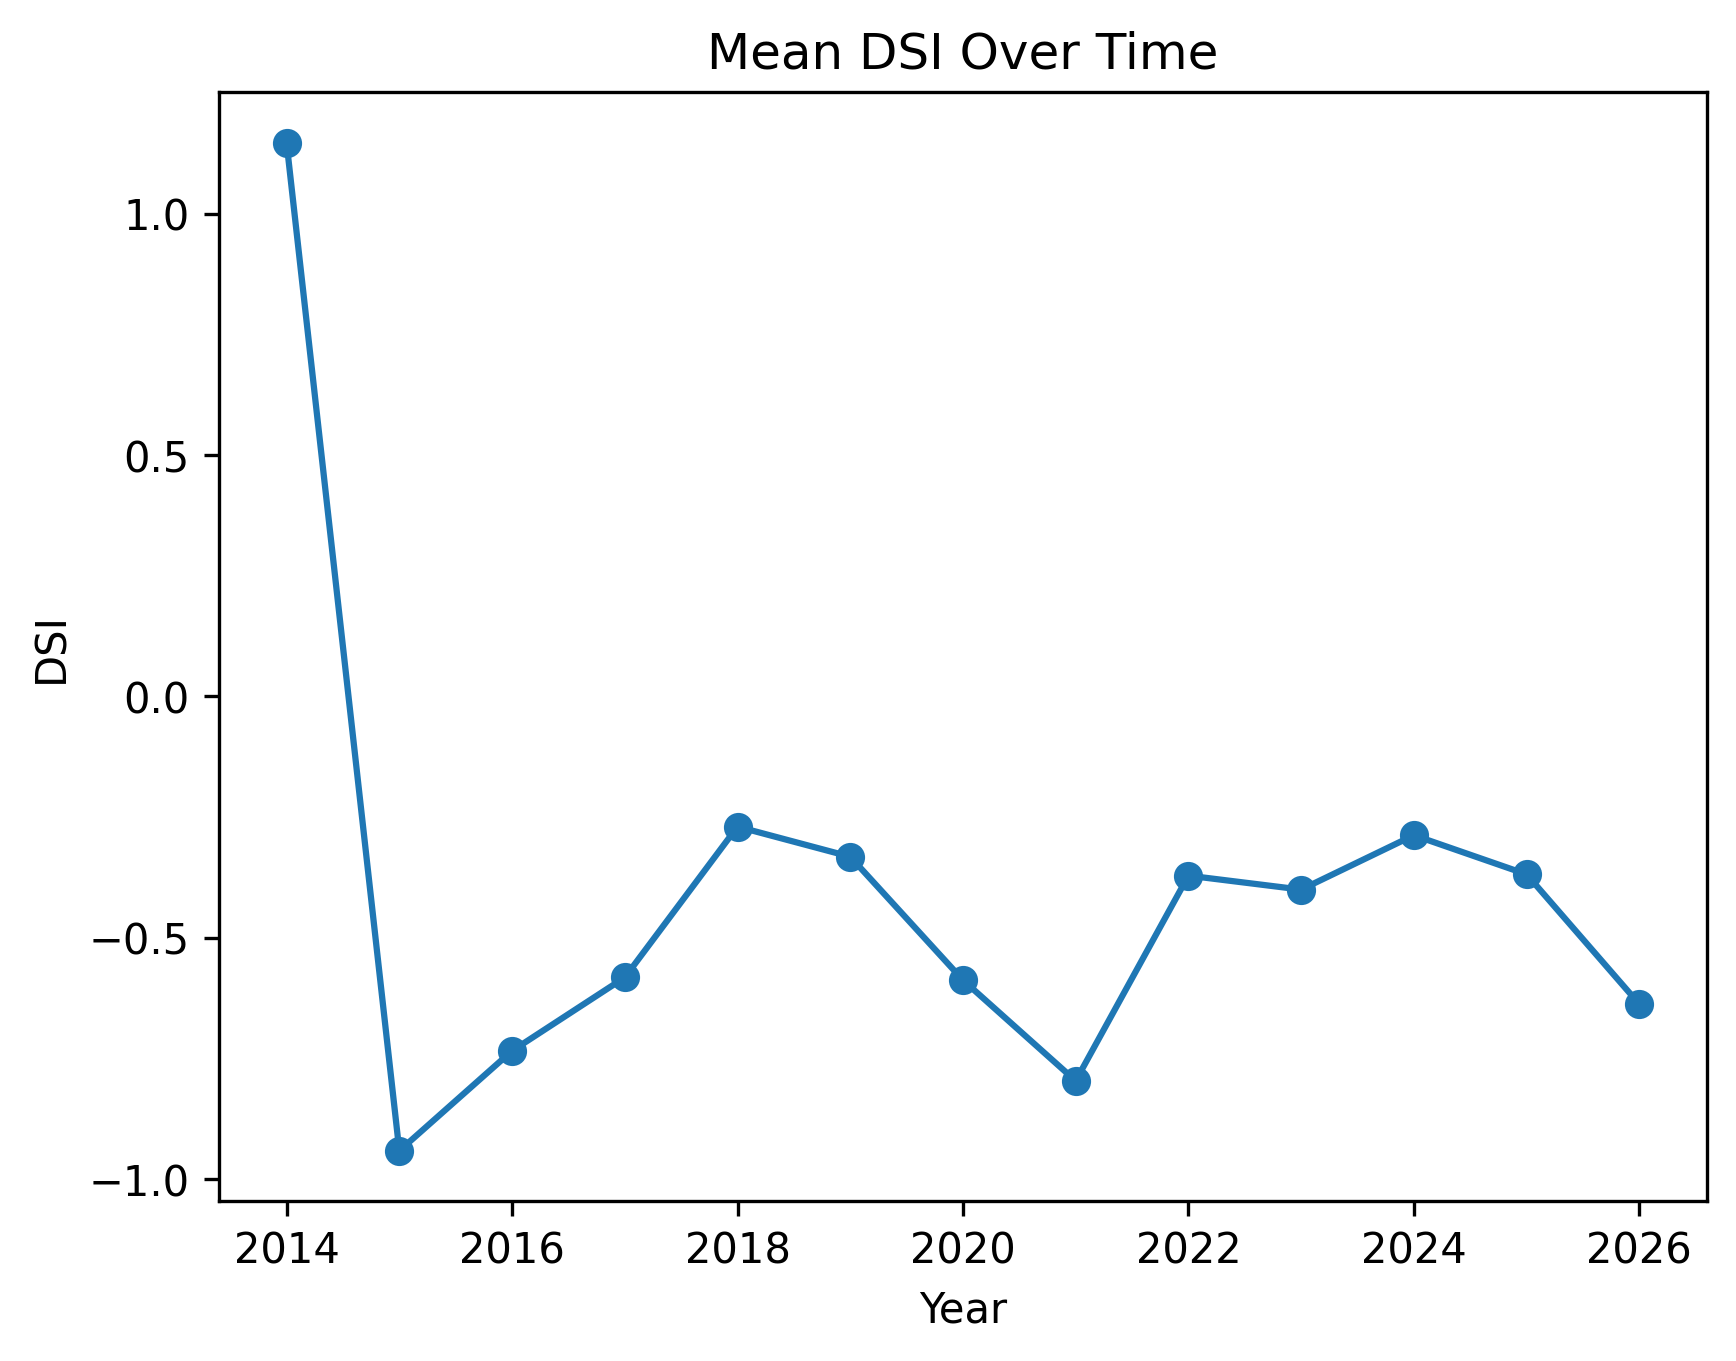
\includegraphics[width=\textwidth]{figures/year-effects.png}

\caption{Temporal trends in DSI}

\end{figure}



\begin{figure}[H]

\centering

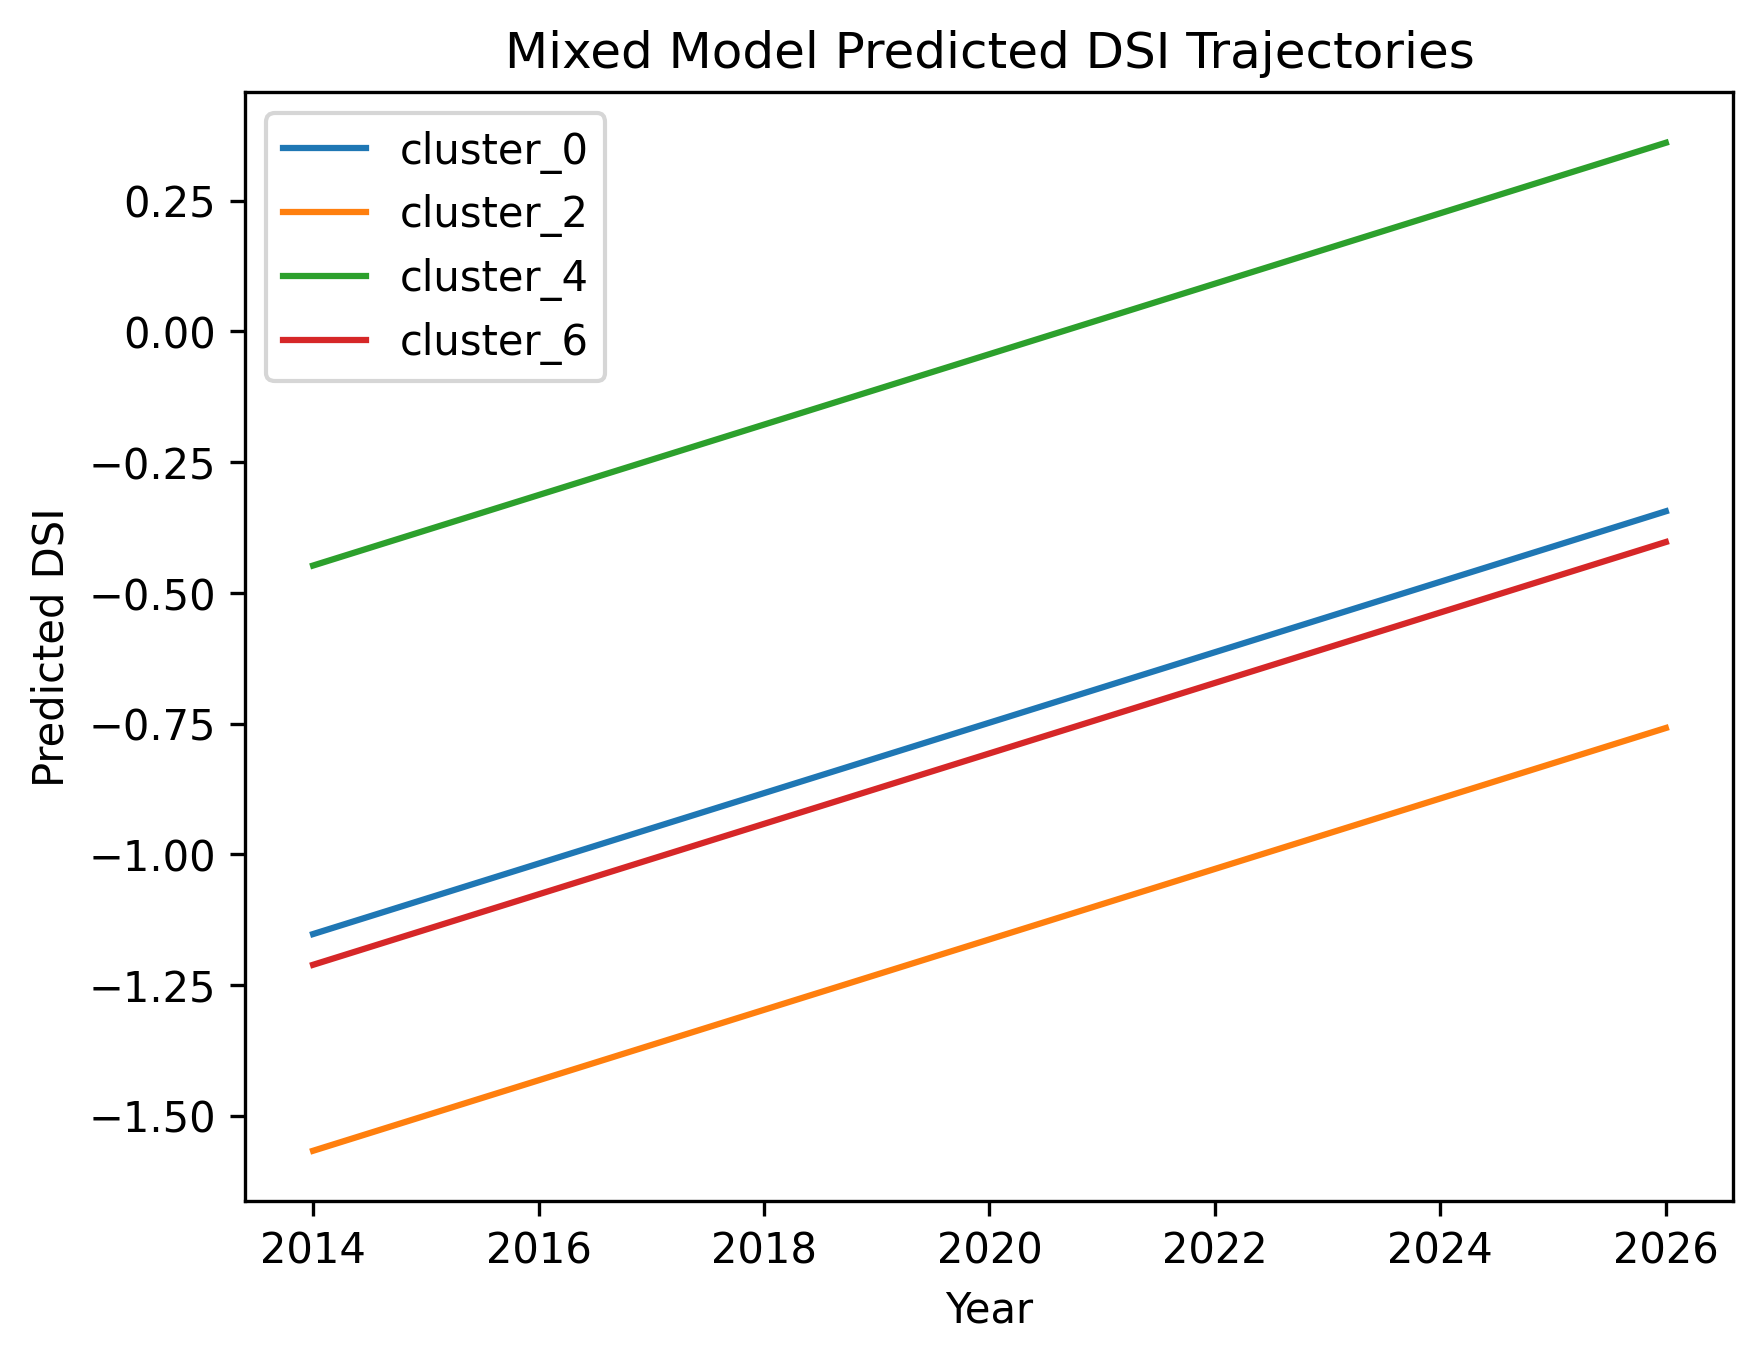
\includegraphics[width=\textwidth]{figures/mixed-effects.png}

\caption{Mixed-effects model results}

\end{figure}



\begin{figure}[H]

\centering

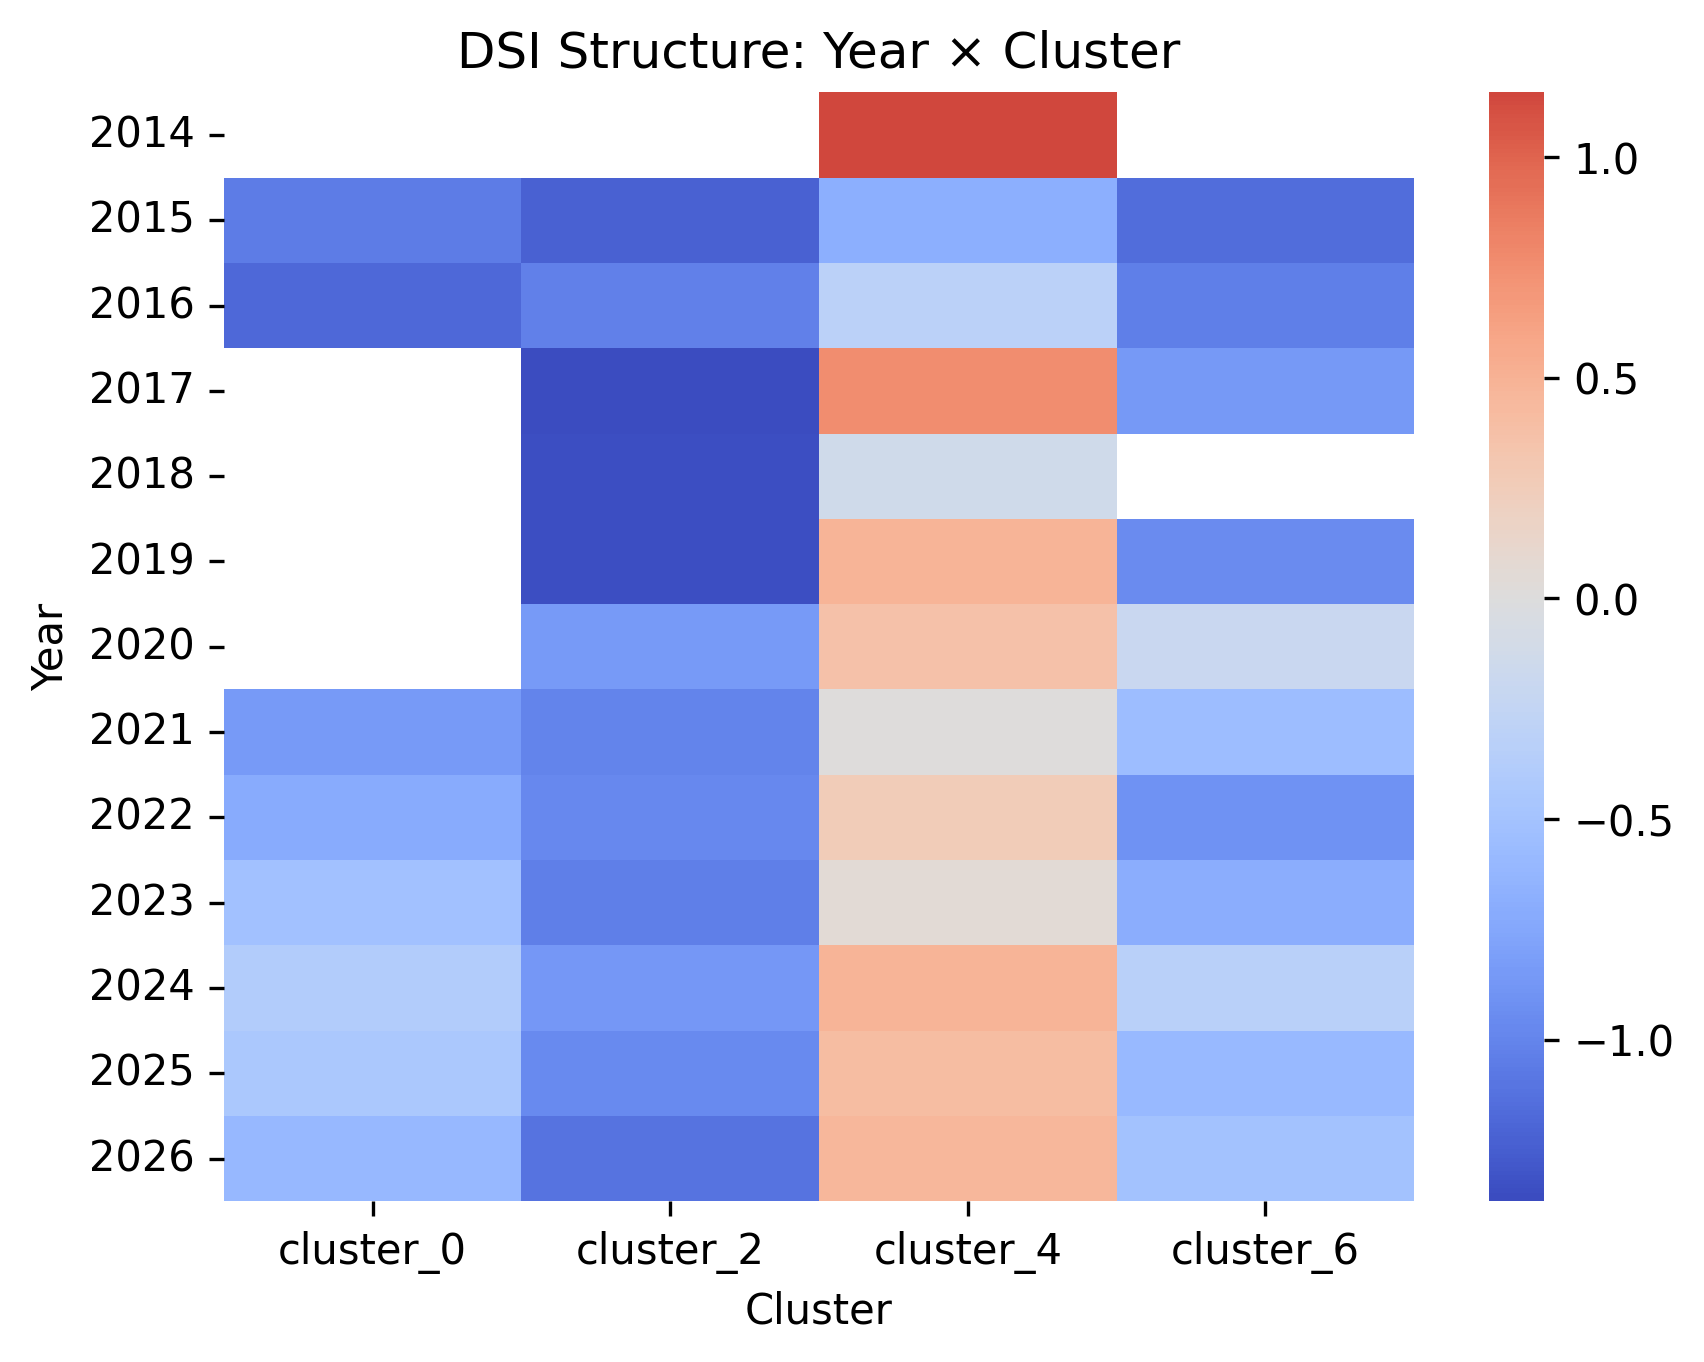
\includegraphics[width=\textwidth]{figures/heatmap.png}

\caption{Cluster-year structure}

\end{figure}



\begin{figure}[H]

\centering

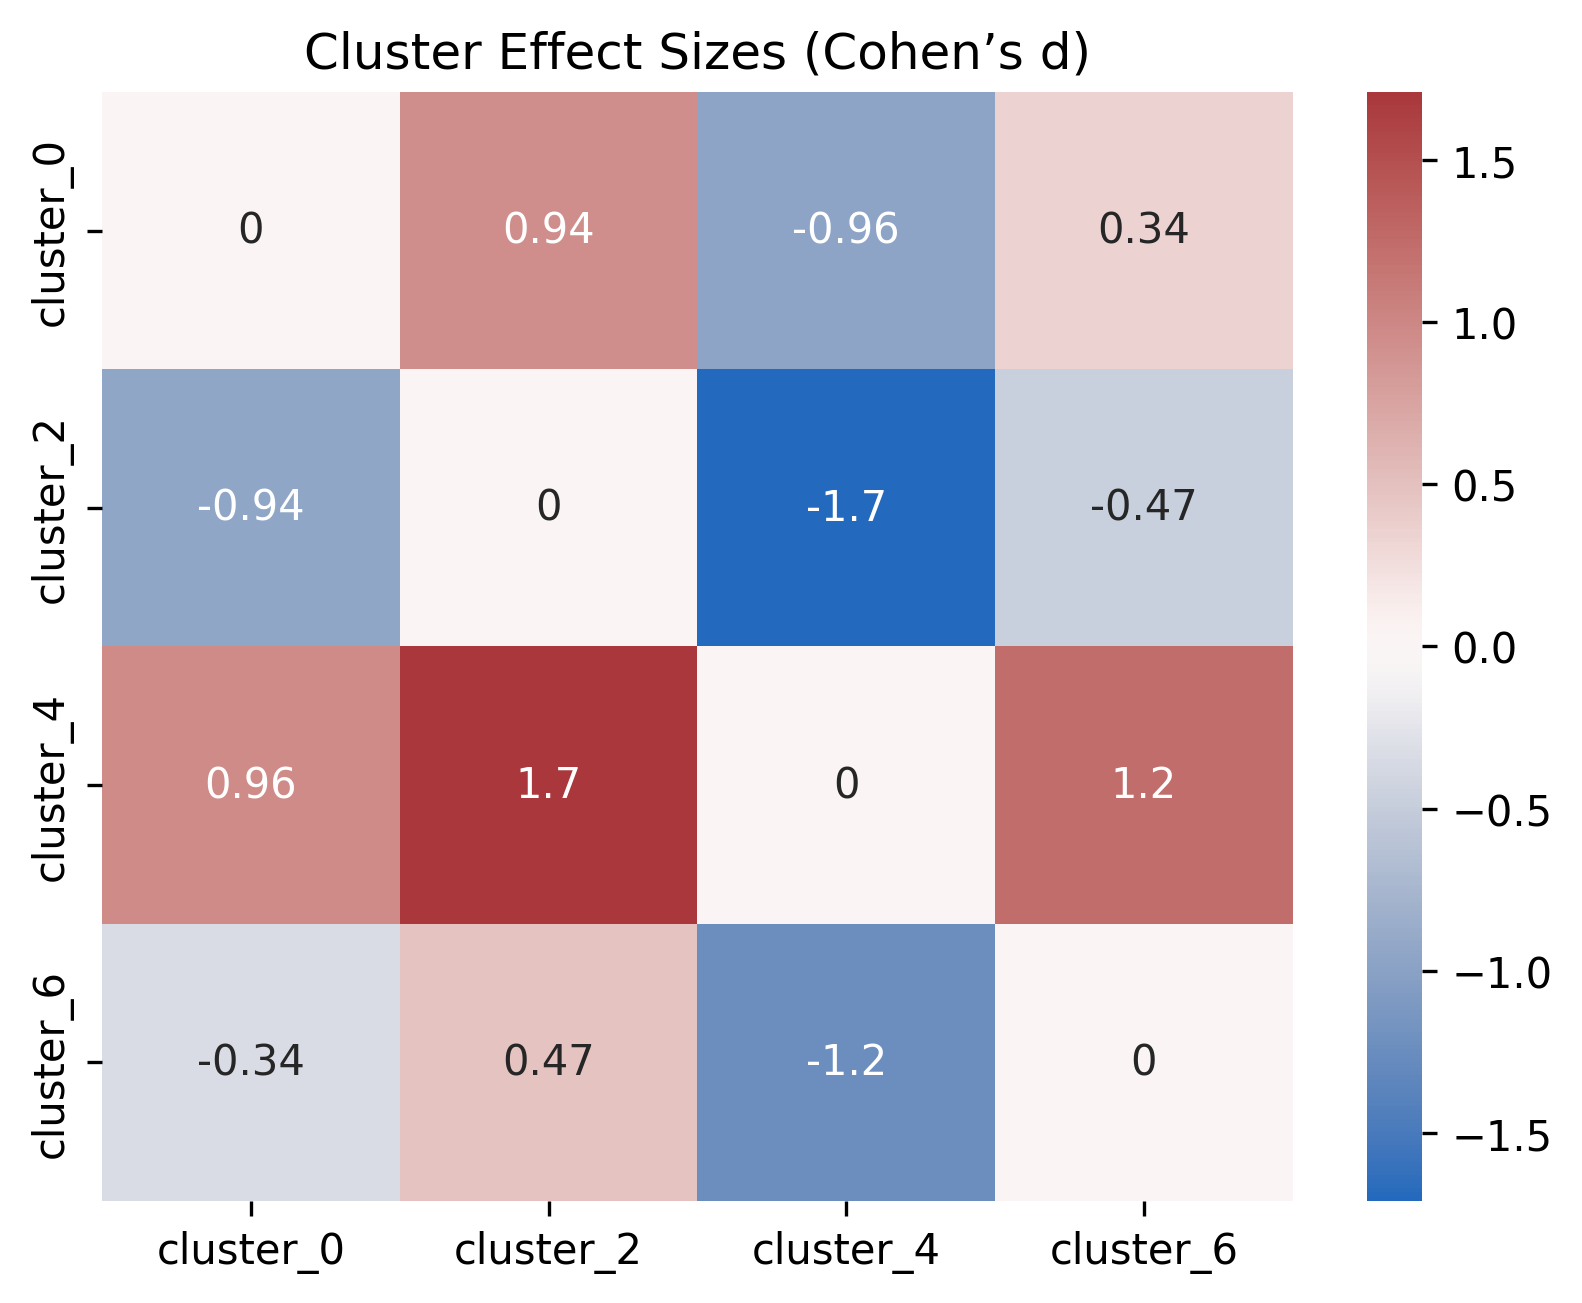
\includegraphics[width=\textwidth]{figures/effect-sizes.png}

\caption{Effect sizes across clusters}

\end{figure}



\ifdraft
  % Do nothing (no bibliography)
\else
  \bibliographystyle{plainnat}
  \bibliography{references}
\fi

\bibliographystyle{unsrtnat}
\bibliography{references}

\end{document}
